\begin{minipage}{0.25\textwidth}
	\centering
	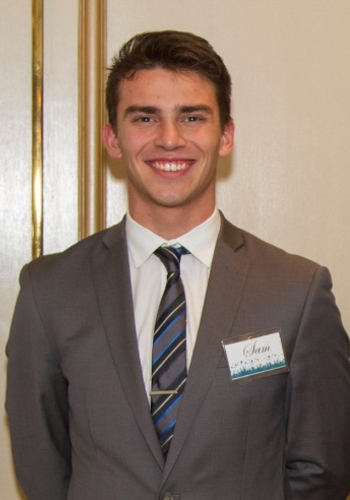
\includegraphics[width=\textwidth]{fmt-dotson.jpg}
\end{minipage}
\begin{minipage}{0.73\textwidth}
	$\textbf{General Co-Chair - Sam Dotson}$\\
Sam graduated with a B.S. in Physics from UIUC in 2019. He attended his first ANS student conference in April 2019 and was so inspired by his experience that he decided to pursue graduate work in nuclear engineering rather than physics. Now he does research on machine learning applications and computational reactor physics with Dr. Kathryn Huff in the ARFC group. Hosting a student conference that will inspire others the way he was inspired is one of his top priorities this year. He has experience planning activities for student organizations such as Guidance for Physics Students (GPS) and has experience fundraising for the College of Lake County (CLC).
\end{minipage}

\begin{minipage}{0.25\textwidth}
	\centering
	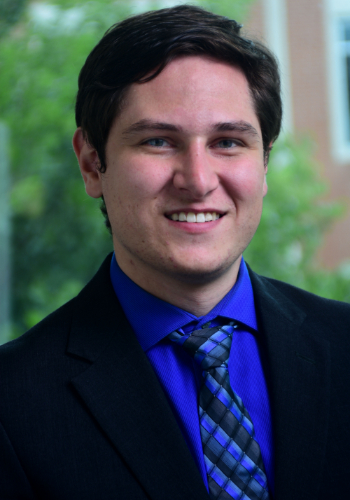
\includegraphics[width=\textwidth]{fmt-mettler.jpg}
\end{minipage}
\begin{minipage}{0.73\textwidth}
	$\textbf{Technical Co-Chair - Jeremy Mettler}$\\
Jeremy graduated with a B.S. in Nuclear, Plasma, and Radiological Engineering from UIUC in 2018, and is now attending as a 3rd-year graduate student studying plasma science under Dr. David Ruzic. He has been heavily involved in the UIUC student chapter of ANS since his freshman year, serving on the executive board for three years as External Vice President and President. Jeremy has attended the past five ANS Student Conferences, which serve as an inspiration for his involvement in this proposal process. He is dedicated to making sure that future generations of students are able to have the same amazing experiences through ANS as he had, especially at the ANS Student Conference. Outside of ANS, he has held a summer internship at Oak Ridge National Lab, and is currently focusing his research towards combined laser-plasma systems for materials processing.
\end{minipage}

\begin{minipage}{0.25\textwidth}
	\centering
	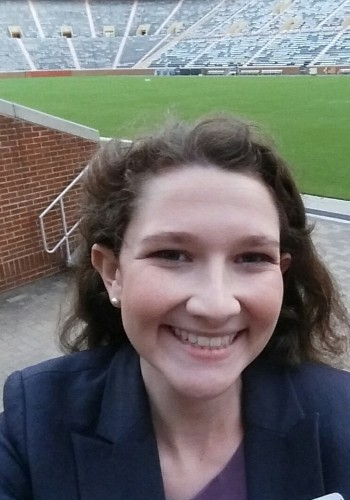
\includegraphics[width=\textwidth]{fmt-bachmanna.jpg}
\end{minipage}
\begin{minipage}{0.73\textwidth}
$\textbf{\textit{Diversity Co-Chair - Amanda Bachmann}}$\\
Amanda has B.S. and M.S. degrees in Nuclear Engineering from the University of Tennessee at Knoxville under Professor Jamie Coble. Now she is a first year PhD student at the University of Illinois where she develops open-source software for nuclear fuel cycle applications with Professor Kathryn Huff. Amanda has served on the ANS Student Sections Committee, the Diversity and Inclusion in ANS Committee, and was recently nominated to be the Student Director on the ANS Board of Directors.
\end{minipage}

\begin{minipage}{0.25\textwidth}
	\centering
	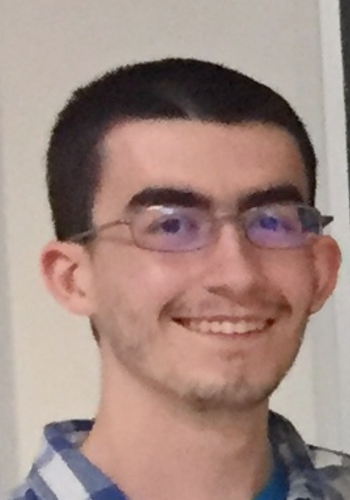
\includegraphics[width=\textwidth]{fmt-armstrongs.png}
\end{minipage}
\begin{minipage}{0.73\textwidth}
	$\textbf{\textit{Financial Chair - Stephen Armstrong}}$\\
Stephen is a junior undergraduate student in UIUC's Nuclear, Plasma, and Radiological Engineering department, with a concentration in Plasma. He serves as the current Finance Chair for ANS-UIUC
\end{minipage}

\begin{minipage}{0.25\textwidth}
	\centering
	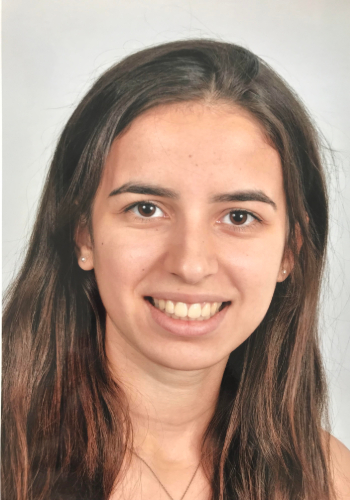
\includegraphics[width=\textwidth]{fmt-dinari.jpg}
\end{minipage}
\begin{minipage}{0.73\textwidth}
	$\textbf{Registration Coordinator - Jasmine Dinari}$\\
Jasmine is a sophomore studying Nuclear, Plasma, and Radiological Engineering at UIUC, as well as minors in French and Physics. She is starting research with Dr. Andruczyk, who is currently at the head of the HIDRA project. Powering the world through nuclear is one of her main interests, and she later hopes to participate in nuclear fusion research. The ANS Student Conference is an  amazing opportunity to share her interests in nuclear science. She gained organizational and leadership experience through various extracurriculars in high school and currently serves as the Professional Development Chair for the UIUC student chapter of Women in Nuclear.
\end{minipage}

\begin{minipage}{0.25\textwidth}
	\centering
	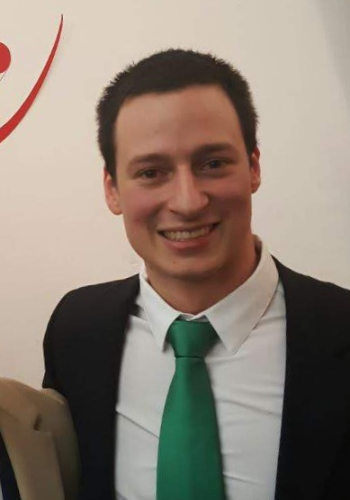
\includegraphics[width=\textwidth]{fmt-fairhurst.jpg}
\end{minipage}
\begin{minipage}{0.73\textwidth}
	$\textbf{Workshops Coordinator - Roberto Fairhurst}$\\
Roberto graduated with a B.S. in Nuclear Engineering from Instituto Balseiro (Argentina) April 2018. He is now a 3rd-year graduate student at UIUC. He does research on computational multi-physics solvers applied to advanced reactors as part of the Advanced Reactors and Fuel Cycle group under the supervision of Dr. Kathryn Huff. He got experience in the organization of conferences during the planning and development of a technical workshop (TWOFCS19) that took place at UIUC in June 2019. His motivation for hosting a student conference is his passion for Nuclear Energy and his desire to transmit this passion to other students. He believes hosting the student conference at UIUC will help the field grow and thrive. This is also an opportunity to meet other people working in the field, share life experiences, and develop a stronger network.
\end{minipage}

\begin{minipage}{0.25\textwidth}
	\centering
	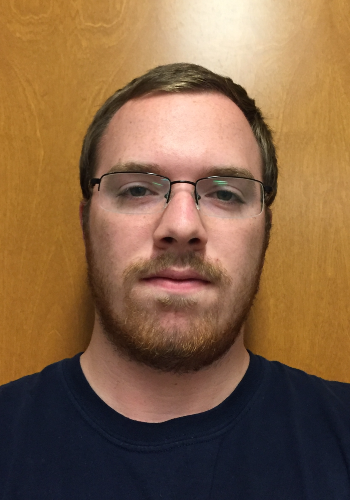
\includegraphics[width=\textwidth]{fmt-hoffmanj.png}
\end{minipage}
\begin{minipage}{0.73\textwidth}
$\textbf{\textit{Sessions Coordinator - Joshua Hoffman}}$\\

\end{minipage}

\begin{minipage}{0.25\textwidth}
	\centering
	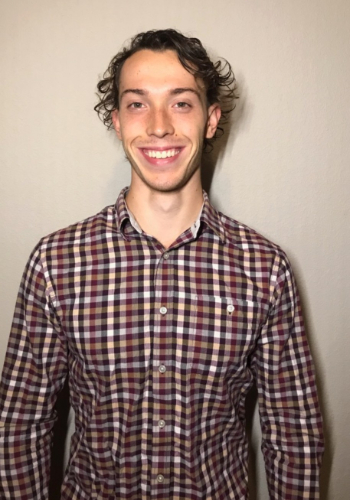
\includegraphics[width=\textwidth]{fmt-golba.jpg}
\end{minipage}
\begin{minipage}{0.73\textwidth}
$\textbf{Career Fair Coordinator - Grzegorz Golba}$\\
	Grzegorz Golba is a sophomore pursuing a B.S. in Nuclear Engineering with a physics minor in the plasma and fusion science concentration. He is now studying material interactions with plasma under Dr. Daniel Andruczyk. Grzegorz attended the 2019 ANS Student Conference in Virginia, reaffirmed his desire to study of nuclear science. He seeks new opportunities to engage with the nuclear science community and is excited for the possibilities of hosting a student conference at UIUC.
\end{minipage}

\begin{minipage}{0.25\textwidth}
	\centering
	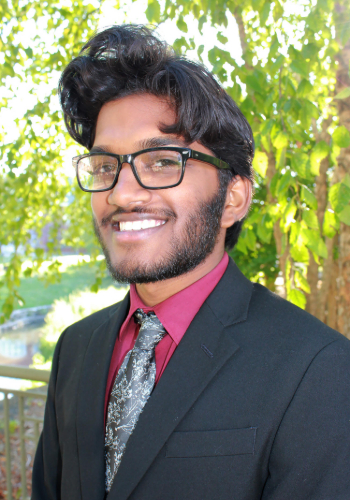
\includegraphics[width=\textwidth]{fmt-dilan.jpg}
\end{minipage}
\begin{minipage}{0.73\textwidth}
	$\textbf{Program Coordinator - Dilan Kurukulasuriya}$\\
Dilan Kurukulasuriay is a sophomore pursuing a B.S. in Nuclear, Plasma, and Radiological Engineering, along with a minor in Physics and Mathematics. He has been active in ANS at UIUC since the start of his freshman year, and he currently serves as the Outreach Chair on the Executive Board. Dilan has worked at the Center for Plasma-Material Interactions lab since the start of his freshman year on HIDRA, and he stayed on campus over the summer to continue to do so. Dilan attended the 2019 ANS Student Conference and it was the highlight of his freshman year of college. He is interested in fusion science research, specifically the materials interaction aspect. He also plans on attending the upcoming student conference at NC State in 2020.
\end{minipage}

\begin{minipage}{0.25\textwidth}
	\centering
	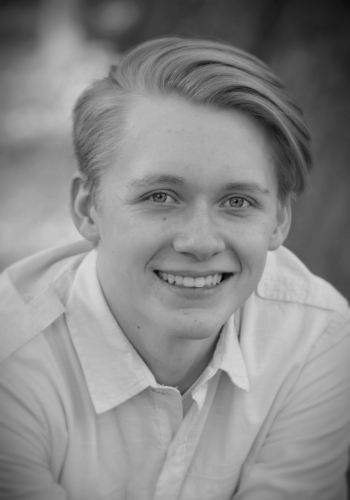
\includegraphics[width=\textwidth]{fmt-davis.jpg}
\end{minipage}
\begin{minipage}{0.73\textwidth}
$\textbf{Hotels and Transportation Coordinator - Gavin Davis}$\\
	Gavin is currently pursuing a B.S. in Nuclear, Plasma, and Radiological Engineering from UIUC and plans to graduate in 2022. He has been involved with the ANS-UIUC since his freshman year and has dedicated his time to outreach events and increasing public awareness of nuclear science and nuclear energy. He has accomplished this through events such as UIUC's Engineering Open House. It was an event he enjoyed as a kid and hopes to help other children develop an interest in nuclear sciences. He also returns to his high school to talk about his experience at UIUC. He looks forward to learning more about nuclear fission technology and to make advancements in nuclear science and in the nuclear energy sector as a whole. He looks forward to attending the student conference at NC State in 2020.
\end{minipage}

\begin{minipage}{0.25\textwidth}
	\centering
	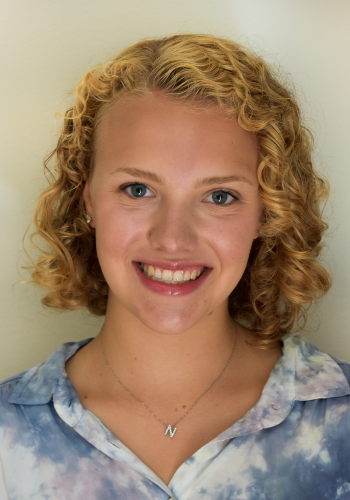
\includegraphics[width=\textwidth]{fmt-panczykn.png}
\end{minipage}
\begin{minipage}{0.73\textwidth}
	$\textbf{\textit{Hospitality and Catering Coordinator - Nataly Panczyk}}$\\
	Nataly is a freshman in Nuclear, Plasma, and Radiological Engineering at UIUC.
\end{minipage}

\begin{minipage}{0.25\textwidth}
	\centering
	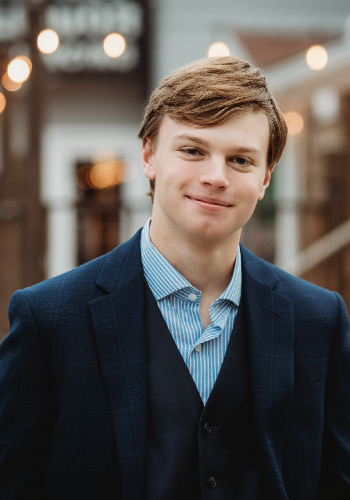
\includegraphics[width=\textwidth]{fmt-mitstiferj.png}
\end{minipage}
\begin{minipage}{0.73\textwidth}
	$\textbf{\textit{Tours Coordinator - Jake Mitstifer}}$\\

\end{minipage}

\begin{minipage}{0.25\textwidth}
	\centering
	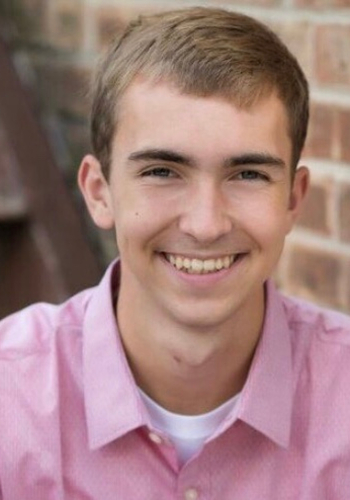
\includegraphics[width=\textwidth]{fmt-ryan.jpg}
\end{minipage}
\begin{minipage}{0.73\textwidth}
$\textbf{Media Coordinator - Nathan Ryan}$\\
	Nathan is pursuing a B.S. in Physics from UIUC. He graduated in the top five of his high school class, while holding down a part time managerial position and running a research project at Argonne National Laboratory concurrent with his Sophomore through Senior years of Secondary Education. His first experience with Nuclear Physics was at the National Superconducting Cyclotron Laboratory where he worked with grad students on rare Cadmium isotopes. He has experience with building appealing website pages, as well as social media communications. He believes that an online presence for this event will supplement the success of an already great set of programs and individuals involved. He is excited to attend the upcoming ANS Student Conference at NC State in 2020.
\end{minipage}
